% !TEX root = ../../技术文档.tex
\section{工程成果}

\subsection{硬件成果}

CPU模块提供可配置单/双发射的六级流水线、两路组相联I/D Cache、动态分支预测和机器异常中断；人脸检测应用采用单发射控制配置，以片上程序和数据存储承担帧任务调度。
NPU完成普通卷积、深度卷积、辅助算子和DMA，并由硬件执行模型计算图；Video完成原图采集、双线性缩放及补边、BGR NCHW输入组织、原图行缓冲、检测框绘制及透明头像合成。
SoC通过AXI连接处理单元、视频DMA和DDR，板级封装统一管理时钟、复位及接口。


\subsection{软件成果}

软件由启动程序、采集与显示驱动、NPU整帧任务驱动、检测后处理和帧池管理组成。
模型工具组织计算图程序、INT8权重、量化参数、CPU解码表及张量布局；硬件UART装载器接收六段模型数据和一段RGBA头像，完成写入确认与CRC校验后封存。
CPU轮询采集、计算和显示事件，在NPU完成后读取九个输出头，执行阈值筛选、框解码和非极大值抑制，再提交同帧显示记录。
异常信息保存在片上SRAM，应用停止提交后续任务并保留现场。


\subsection{功能验证}

CPU与NPU组件验证、底层互连接口验证、Video独立板测分别使用各自配置；CPU独立CoreMark采用100\,MHz，Video三模式演示使用独立顶层。
头像应用的融合仿真采用50/125/40\,MHz时钟和实际应用固件，DDR端点为存储代理，验收摘要见表\ref{tbl:box-system-summary}。
两组场景均核对九头输出、完整画面、同帧身份及旧槽释放复用，详细事件计数见附录\ref{sec:box-system-validation}。
数值参考与硬件采用相同的输入、量化和后处理规则。

\begin{reporttable}
\begin{longtable}{@{}p{0.22\linewidth}p{0.48\linewidth}p{0.23\linewidth}@{}}
\caption{头像应用融合仿真验收摘要}\label{tbl:box-system-summary}\\
\toprule
场景 & 通过内容 & 依据 \\
\midrule
\endfirsthead
\caption[]{头像应用融合仿真验收摘要（续）}\\
\toprule
场景 & 通过内容 & 依据 \\
\midrule
\endhead
\bottomrule
\endfoot
自然人脸 & 两帧均输出1脸，RAW、BOX、AVATAR逐像素核对，旧槽经确认后复用 & 附录F自然人脸回归 \\
零RGB空场景 & 两帧均输出0脸，三模式均保持原图，旧槽经确认后复用 & 附录F零RGB回归 \\
\end{longtable}
\end{reporttable}


\subsection{应用演示}

\noindent\textbf{人脸检测与头像叠加应用}\par

应用接入800$\times$600、标称60\,Hz的HDMI视频，经过原图采集、模型输入预处理、NPU整图推理和CPU后处理，按选择的模式输出原图、检测框或透明头像。
CPU从保留的检测框中按面积、分数和候选序号选择主人脸，头像覆盖区域随主框位置和尺寸更新；无脸时显示原图。CPU/NPU运行于50\,MHz，Video/DDR用户接口运行于125\,MHz，输出像素时钟为40\,MHz。

作品实物及视频演示环境如图\ref{fig:system-overview-photo}所示。
中央笔记本提供HDMI视频输入，右下方的开发板完成视频处理，左侧显示器展示叠加人脸检测框后的画面。

\begin{figure}[!htbp]
\centering
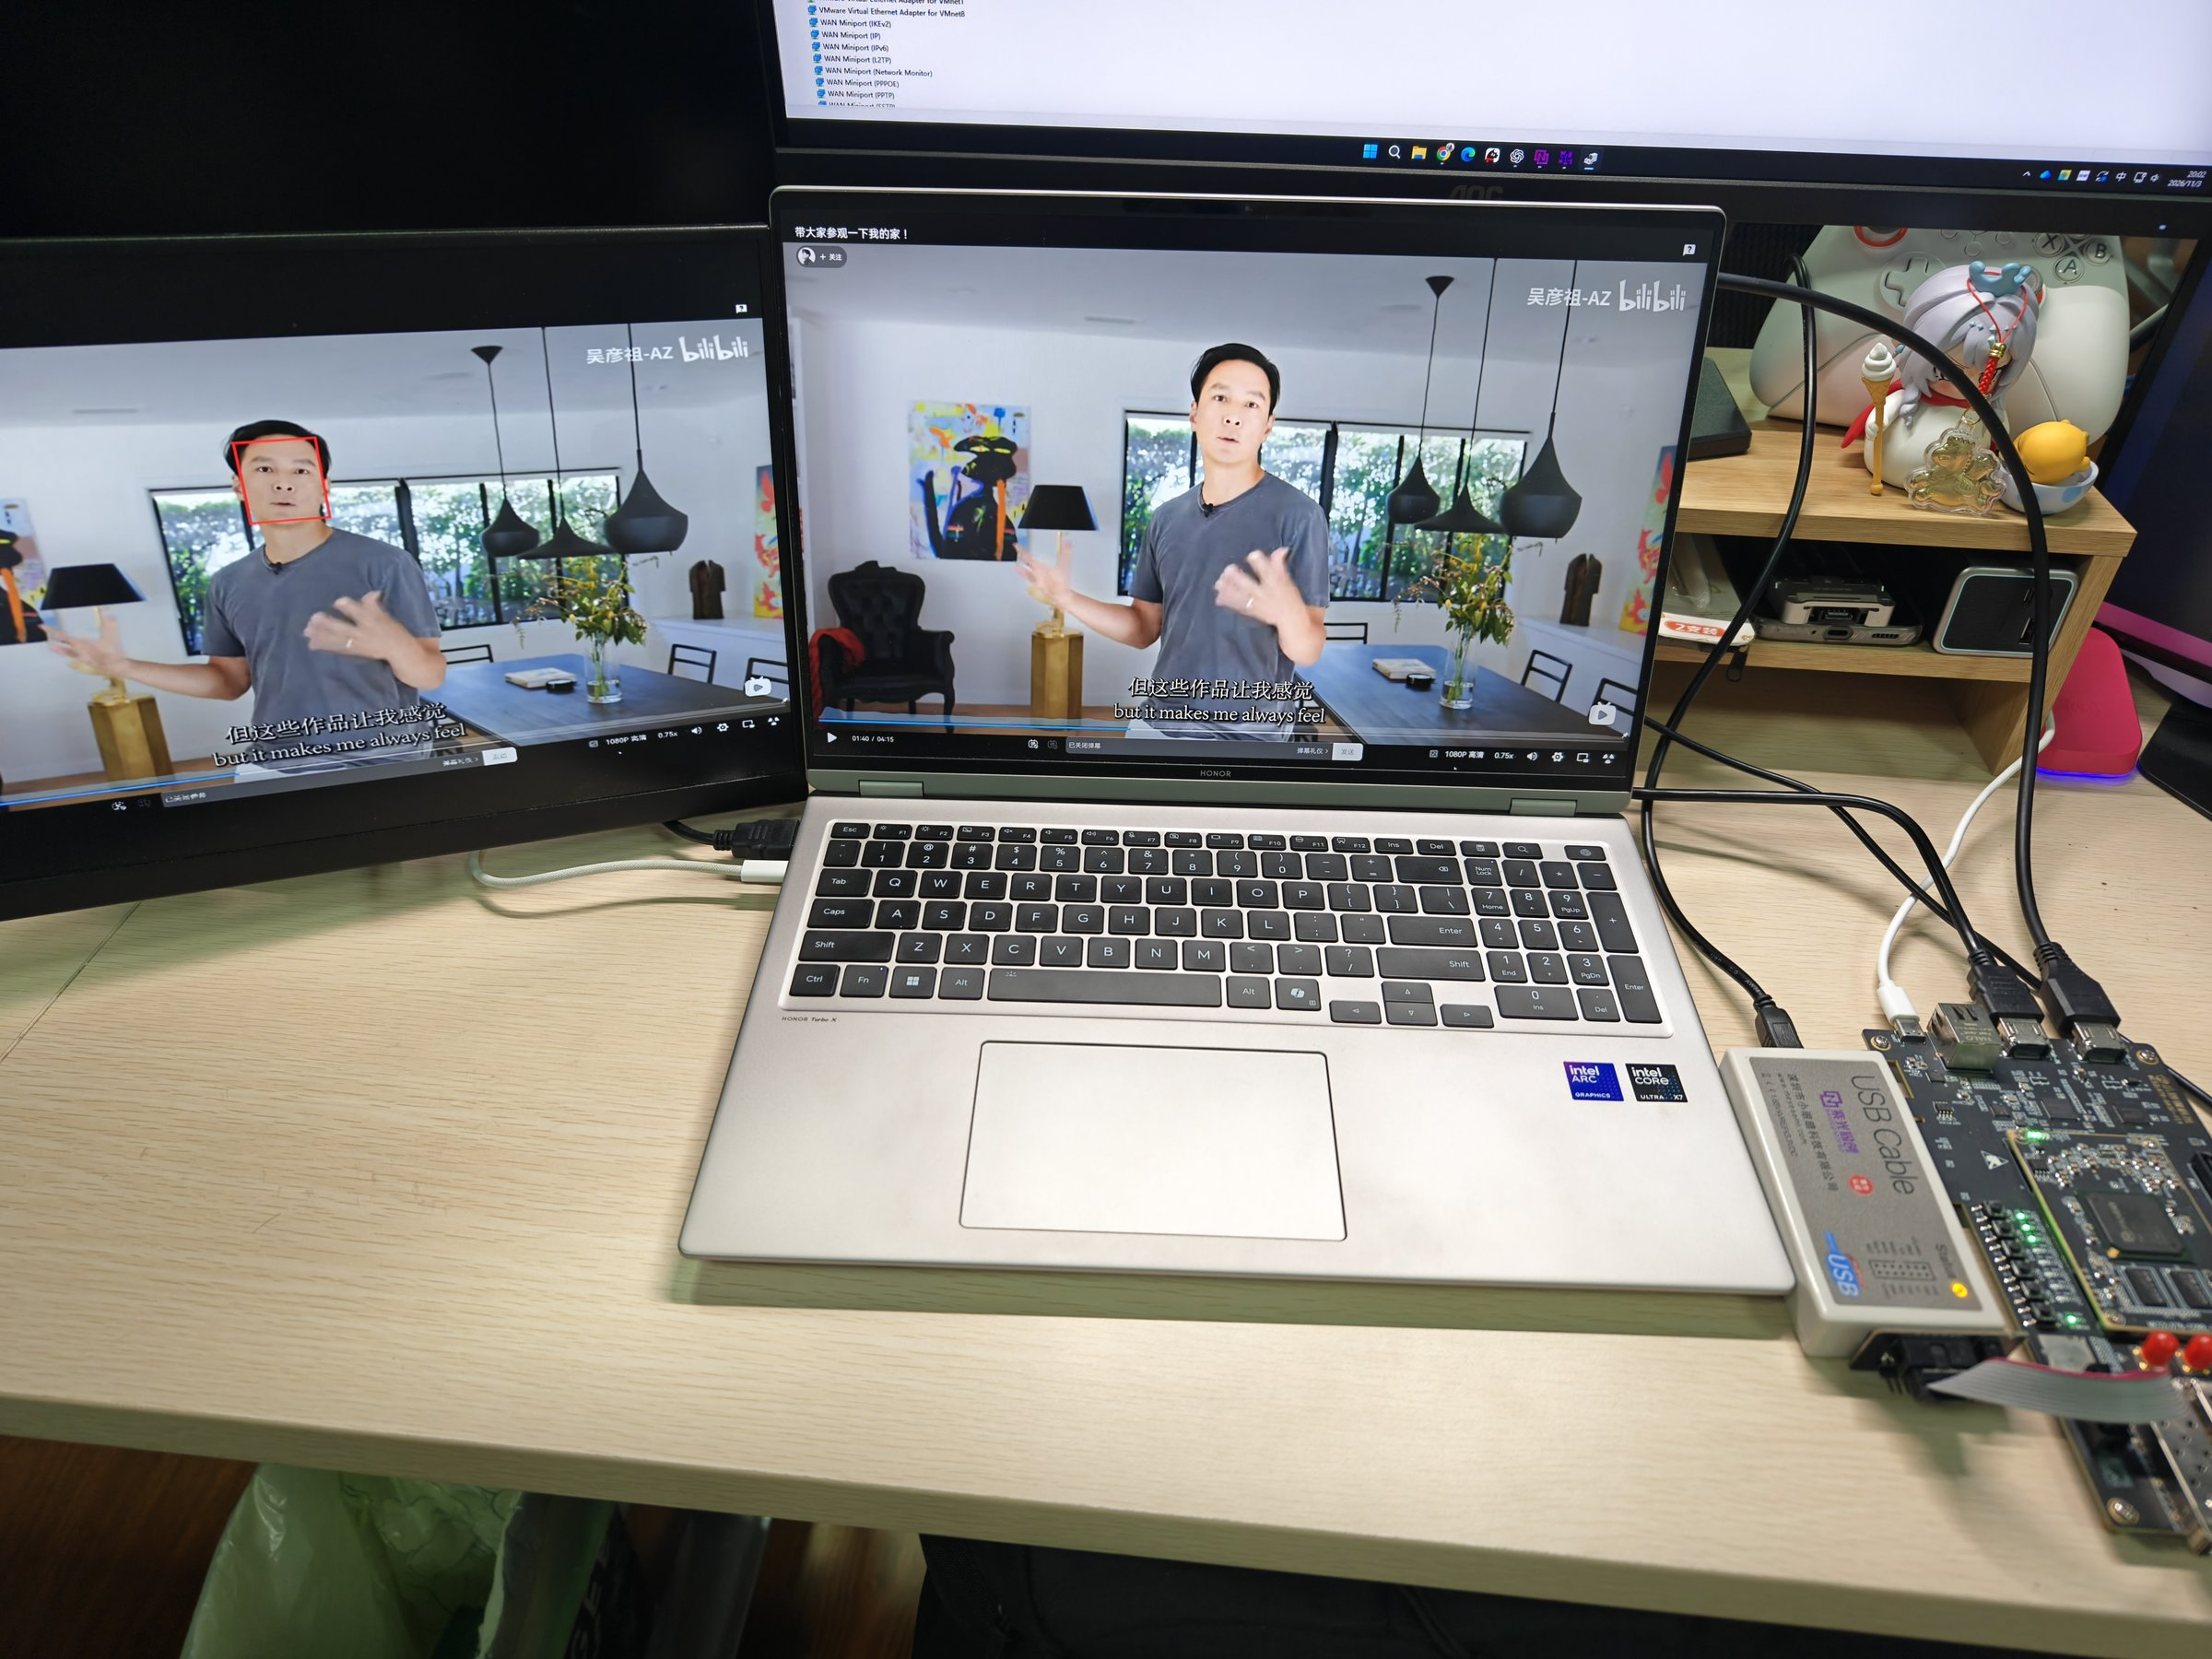
\includegraphics[width=0.69\linewidth]{../figure/triha-system-overview-photo.jpg}
\caption{TriHaRiscv作品全景}\label{fig:system-overview-photo}
\end{figure}

开发板的JTAG Program/Verify及七段模型和头像装载均通过。传输共2,032,640\,B、7,940包，重传0次，最终确认游标为$(7,0)$，随后完成封存。
现场通过HDMI输出确认了三模式切换、头像随人脸位置和尺寸更新、透明区域显示背景、无脸时清除及人脸返回后恢复，结果见表\ref{tbl:face-box-board-results}。

\begin{reporttable}
\begin{longtable}{@{}p{0.24\linewidth}p{0.30\linewidth}p{0.38\linewidth}@{}}
\caption{人脸检测与头像叠加板测结果}\label{tbl:face-box-board-results}\\
\toprule
检查项目 & 结果 & 验证方式与范围 \\
\midrule
\endfirsthead
\caption[]{人脸检测与头像叠加板测结果（续）}\\
\toprule
检查项目 & 结果 & 验证方式与范围 \\
\midrule
\endhead
\bottomrule
\endfoot
配置下载与校验 & Program / Verify通过 & PG2L100H易失JTAG配置 \\
模型及头像装载 & 七段传输与封存通过 & 7,940包，0重传，最终游标$(7,0)$ \\
模式切换 & RAW、BOX、AVATAR正常 & KEY1逐次切换并观察HDMI输出 \\
头像跟随 & 随人脸位置和尺寸更新 & 改变人脸位置及大小 \\
透明合成 & 透明像素处可见背景 & 核对输入照片的透明区域 \\
无脸与恢复 & 头像消失，人脸返回后恢复 & 现场移除和重新引入人脸 \\
\end{longtable}
\end{reporttable}

上述板测记录用于功能验收。配置、模型和头像采用易失装载，断电后重新执行JTAG配置和七段数据上传。
115200\,baud、8N1下，仅有效载荷的理论传输时间约为176.4\,s；含包头和确认包的线速预算约为195.7\,s，实际装载历时没有记录。
本次验收也未记录明确窗口内的完成结果数和新帧首次显示数，实际应用板级帧率尚未测得。

\noindent\textbf{Video独立三模式验证}\par

Video独立板级验证使用\texttt{video\_live\_mode\_board}目标，接入动态HDMI源，核对三种模式的连续背景、按键切换及协调复位。
BOX使用人工生成的框和关键点，AVATAR使用256$\times$256 RGBA算术测试纹理。
这些输入用于检查视频数据通路、模式控制与逐像素合成，板测数据见表\ref{tbl:video-board-results}。

\begin{reporttable}
\begin{longtable}{@{}p{0.24\linewidth}p{0.30\linewidth}p{0.38\linewidth}@{}}
\caption{Video独立板级验证结果}\label{tbl:video-board-results}\\
\toprule
检查项目 & 结果 & 统计范围 \\
\midrule
\endfirsthead
\caption[]{Video独立板级验证结果（续）}\\
\toprule
检查项目 & 结果 & 统计范围 \\
\midrule
\endhead
\bottomrule
\endfoot
图像与时钟 & 800$\times$600；40/125\,MHz & 输出像素时钟/核心时钟 \\
显示扫描频率 & 约60.32\,Hz & 1056$\times$628光栅 \\
新图更新率 & 30.1548\,fps & 复位后84\,s生命周期采样窗口 \\
连续健康观察 & 87.000\,s & 复位后的持续观察时长 \\
模式与复位 & 三次模式切换、一次复位通过 & KEY1循环三模式，KEY0恢复RAW \\
欠载、溢出及错误 & 均为0 & 已记录的连续三模式及复位观察 \\
LUT / FF & 16770 / 18150 & 整个独立Video板级目标 \\
片上存储 & 73.5个DRM36K等效块 & 含64个测试纹理缓存块 \\
Slow setup / hold & +0.063 / +0.129\,ns & 实际后布线时序报告 \\
Fast setup / hold & +2.911 / +0.097\,ns & 实际后布线时序报告 \\
配置下载与校验 & Program / Verify通过 & 与时序报告对应的板级镜像 \\
\end{longtable}
\end{reporttable}

板测记录与机器证据保存于\path{docs/verification/video/live_modes.md}及其关联证据文件。
新图更新率按采集帧标识变化计数；扫描频率按输出光栅计数。
表中30.1548\,fps对应独立Video目标的采集与显示生命周期，不计入真实人脸检测应用的推理性能。


